\section{Paper 5 highlights: Identifying levers for improving thrombolysis use and outcomes – combining clinical pathway simulation and machine learning applied to the UK stroke registry.\cite{pearn_identifying_2024}} \label{sec:paper_5}

\subsection{Objective}

By combining clinical pathway simulation and machine learning of thrombolysis decision-making and outcomes, we sought to better understand the source of variation in thrombolysis use and the effect on outcomes. We also sought to investigate the cost-effectiveness of thrombolysis in stroke teams with lower or higher thrombolysis use.

\subsection{Methods overview}

\subsubsection{Models}

This work combined four models:

\begin{enumerate}

    \item \textit{Thrombolysis decision model}: An XGBoost machine learning model \cite{chen_xgboost_2016} was used to learn which patients would receive thrombolysis at each stroke team. Stroke team SHAP values were used to identify 25 \textit{benchmark teams} most likely to use thrombolysis. For each patient a \textit{benchmark decision} was predicted, which was the majority vote of the expected decision for that patient at the 25 \textit{benchmark teams}. This is based on the model as described in section %\ref{sec:paper_2}.

    \item \textit{Outcome model}: A XGBoost machine learning model was used to predict outcome (mRS probability distribution) for each patient. This is based on the model as described in section %\ref{sec:paper_4}.

    \item \textit{Patient pathway flow}: Monte-Carlo simulation was used to model the flow of patients through the emergency stroke pathway at each hospital, taking into account both average speeds and variation. When examining the effect of improving patient flow, clinical outcome is predicted as the number of \textit{excellent outcomes} (mRS 0-1) per 1,000 admissions using a previously described mathematical model \cite{allen_estimation_2020}.

    \item \textit{Lifetime economic model}: A model predicting life expectancy, quality-adjusted life years (QALYs), and NHS care costs after stroke, based on age, sex, and disability at discharge\cite{mcmeekin_lifetime_2024}.
    
\end{enumerate}

\subsubsection{Prototype patients}

To help compare decision-making and outcomes across stroke teams we exemplified differences using \textit{prototype patients}. These prototype patients captured a range of features known to affect decisions to treat, and to affect outcomes, and included an \textit{ideal} candidate for thrombolysis. The prototype patients used were:

\begin{enumerate}
    \item \textit{Ideal}: Onset-to-arrival = 90 minutes; arrival-to-scan = 15 minutes; onset-to-thrombolysis = 120 minutes; stroke severity (NIHSS) = 15; pre-stroke disability (mRS) = 0; age = 72.5; precisely known onset; onset not during sleep; stroke type = infarction; patient has no atrial fibrillation and is not receiving anticoagulants for atrial fibrillation.

    \item \textit{Late arrival}: As \textit{ideal} but onset-to-arrival = 225 minutes and onset-to-thrombolysis (when given) = 255 minutes.

    \item \textit{Mild}: As \textit{ideal} but stroke severity = 3.

    \item \textit{Prior disability}: As \textit{ideal} but pre-stroke disability = 3

    \item \textit{Imprecise}: As \textit{ideal} but stroke onset time estimated.

    \item \textit{Age}: As \textit{ideal} but age = 87.5.

    \item Combinations of the above.
\end{enumerate}


\subsubsection{Pathway changes}

The combined model may be used to examine a range of possible changes to improve use of thrombolysis:

\begin{enumerate}

    \item \textit{Base}: Uses the hospitals’ recorded pathway statistics.

    \item \textit{Speed}: Sets 95\% of patients having a scan within 4 hours of arrival (other assumed to be late scan, due to atypical stroke symptoms), and all patients have 15 minutes arrival-to-scan time and 15 minutes scan-to-needle time.

    \item \textit{Ambo}: Subtracts 15 minutes from the current ambulance-call to arrival-at-hospital times.

    \item  \textit{Onset-known}: Sets the proportion of patients with a known stroke onset time to the national upper quartile (79.6\%) if currently less than the national upper quartile.

    \item \textit{Benchmark}: The benchmark thrombolysis rate takes the likelihood to give thrombolysis for patients scanned within 4 hours of onset from the majority vote of the 25 benchmark hospitals (see above).

    \item Combinations of the above.

\end{enumerate}

Code, with demonstration, is available at \url{https://github.com/samuel-book/samuel_2_demo}.


\subsection{Key results}

\subsection{Model accuracy}

Using an 4:1 train:test split, the thrombolysis decision model had an accuracy of 85\%, a balanced accuracy (mean of sensitivity and specificity) of 82\% (accuracy and balanced accuracy using a 50\% probability cut-off to classify a patient as a binary `likely to receive thrombolysis' or not), and a receiver operating characteristic area under curve of 0.92. The stroke outcome model had a receiver operating characteristic area under curve of 0.80.

\subsection{Benchmark stroke teams and benchmark decisions}

\textit{Benchmark decisions} are those that would likely be taken by the majority 25 \textit{benchmark} stroke teams most likely to use thrombolysis (if all stroke teams saw the same patients). If all decisions-to-treat were made according to benchmark decisions, the average thrombolysis rate across stroke teams would increase from 36\% to 45\% (in the modelled patient population). Thrombolysis use in the 25 stroke teams least likely to use thrombolysis would increase from 29\% to 46\%.

Figure \ref{fig:thrombolysis_rates_teams} compares observed and predicted thrombolysis use (based on historic performance, and applying \textit{benchmark decisions}). Predicted and observed thrombolysis use correlate very closely (r-squared 0.94). Predicted rates were, on average, slightly higher (1.7\%) than observed rates.

\begin{figure}
    \centering
    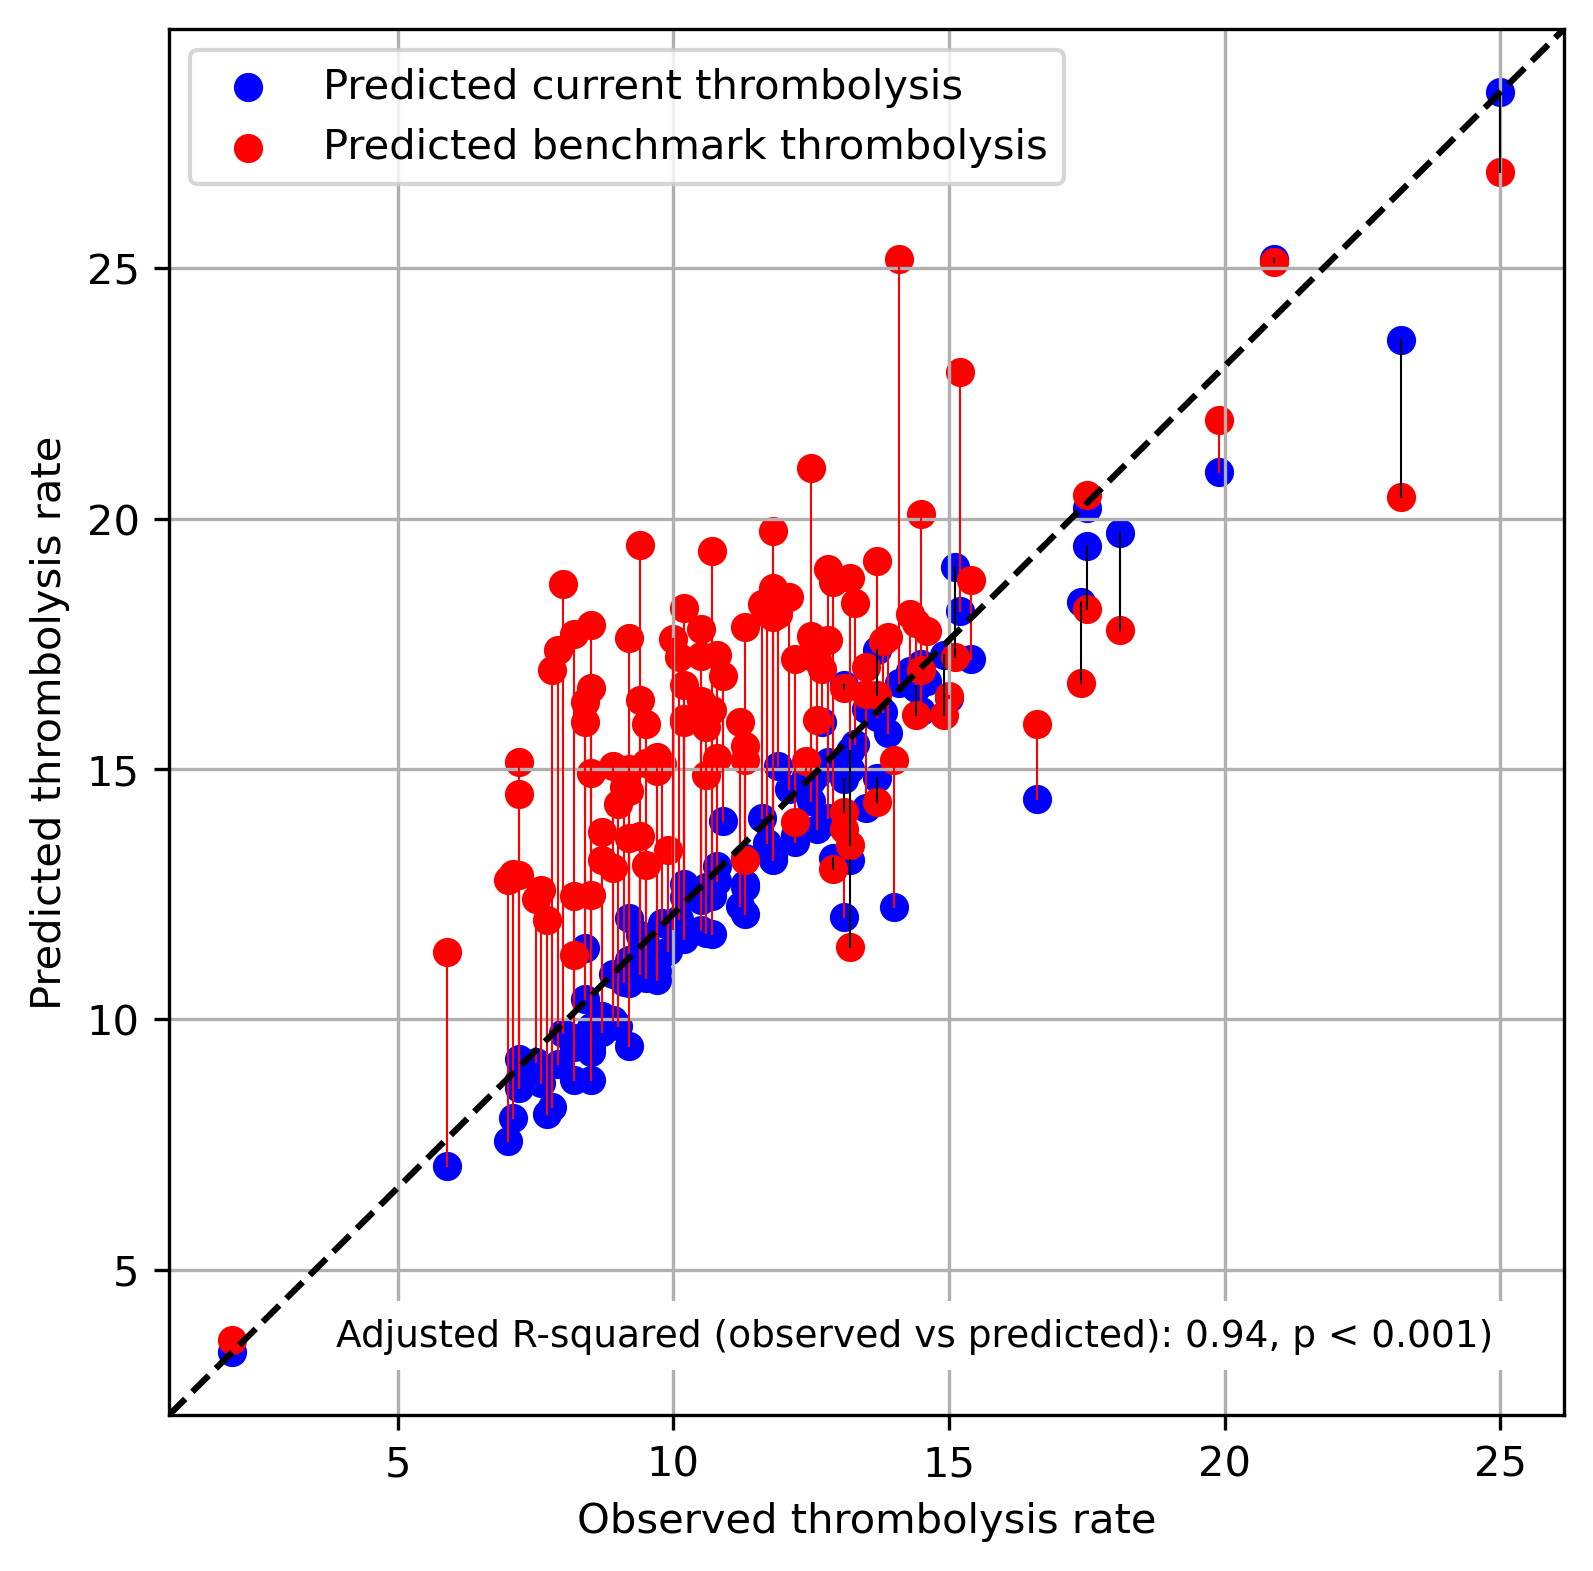
\includegraphics[width=0.5\linewidth]{images/p5_benchmark_rates.png}
    \caption{Comparison of observed and predicted thrombolysis use across stroke teams. Blue circles show predictions based on historic hospital performance. Red circles show the expected thrombolysis use if \textit{benchmark decisions} were made. The black dotted line shows least-squares regression analysis between observed and predicted (using historic performance) thrombolysis use.}
    \label{fig:thrombolysis_rates_teams}
\end{figure}

\subsubsection{Prototype patients}

Prototype patients revealed variation in likely decisions between stroke teams (figure \ref{fig:thrombolysis_rates_prototype_patients}). While almost all stroke teams would give thrombolysis to the \textit{ideal} candidate for thrombolysis, the predicted use of thrombolysis varied more as one characteristic was changed from the \textit{ideal} candidate. In particular there was a very wide range in likelihood of a patient with a mild stroke (NIHSS 3) receiving thrombolysis. Mild stroke (NIHSS 0-4) represents a large proportion of admissions (54\% of all emergency stroke admissions, and 38\% of ischaemic stroke patients arriving by ambulance within 4 hours of known stroke onset). Combinations of \textit{non-ideal} patient characteristics reduced predicted use of thrombolysis further (again with significant variation between stroke teams), especially when the non-ideal characteristic was a mild stroke.

\begin{figure}
    \centering
    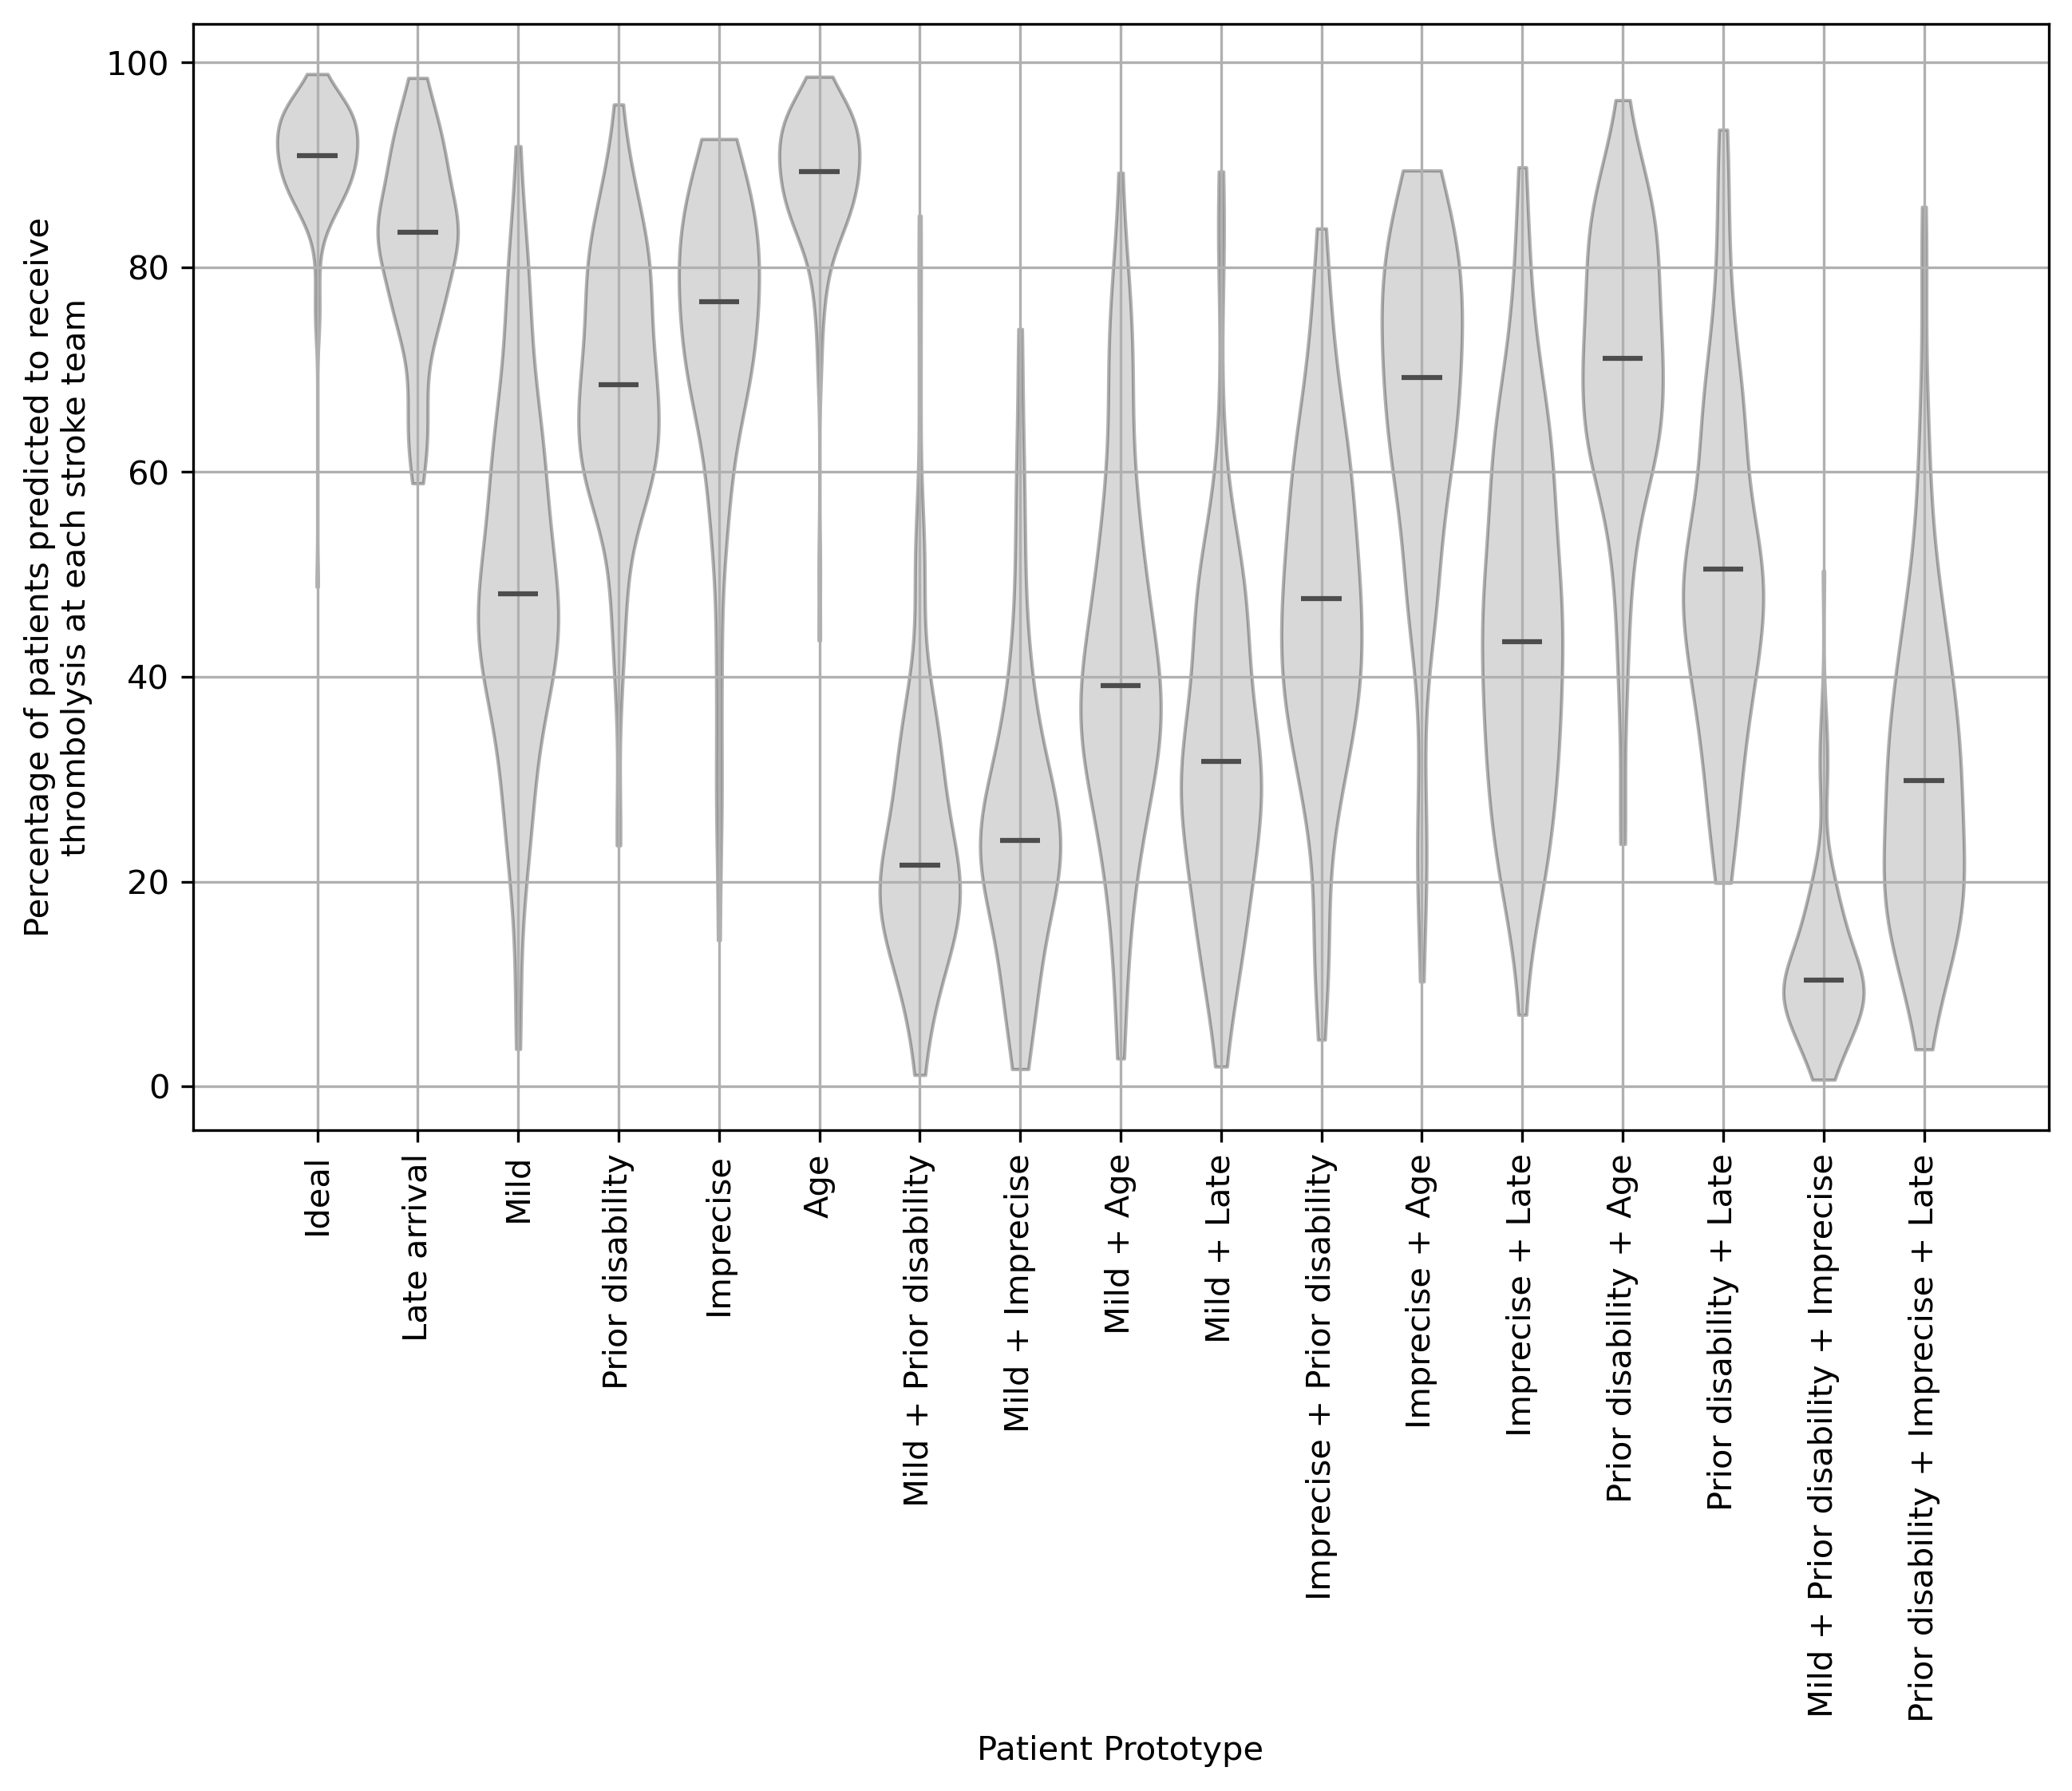
\includegraphics[width=0.75\linewidth]{images/p5_prototype_decision.png}
    \caption{Violin plots showing the variation in predicted thrombolysis rates for 17 patient prototypes across stroke teams. \textit{Ideal}: onset-to-arrival = 90 minutes; arrival-to-scan = 15 minutes; onset-to-thrombolysis = 120 minutes; stroke severity (NIHSS) = 15; pre-stroke disability (mRS) = 0; age = 72.5; precisely known onset; onset not during sleep; stroke type = infarction; patient has no atrial fibrillation and is not receiving anticoagulants for atrial fibrillation; \textit{Late arrival}: as \textit{ideal} but onset-to-arrival = 225 minutes and onset-to-thrombolysis = 255 minutes; \textit{Mild}: As \textit{ideal} but stroke severity = 3; \textit{Prior disability}: as \textit{ideal} but pre-stroke disability = 3; \textit{Imprecise}: as \textit{ideal} but stroke onset time estimated; \textit{Age}: as \textit{ideal} but age = 87.5.}
    \label{fig:thrombolysis_rates_prototype_patients}
\end{figure}

Table \ref{tab:prototype_outcomes} shows predicted outcomes across all prototype patients. All these patients would likely benefit from thrombolysis, but the benefit in mild stroke was smaller.

\begin{minipage}{1\textwidth}
\small
\begin{longtable}{p{5.2cm} | p{1.6cm} p{1.6cm} p{1.5cm} | p{1.6cm} p{1.6cm} p{1.5cm}}
\caption{Predicted outcomes for patient prototypes. \textit{Ideal}: onset-to-arrival = 90 minutes; arrival-to-scan = 15 minutes; onset-to-thrombolysis = 120 minutes; stroke severity (NIHSS) = 15; pre-stroke disability (mRS) = 0; age = 72.5; precisely known onset; onset not during sleep; stroke type = infarction; patient has no atrial fibrillation and is not receiving anticoagulants for atrial fibrillation. \textit{Late arrival}: as \textit{Ideal} but onset-to-arrival = 225 minutes and onset-to-thrombolysis = 255 minutes; \textit{Mild}: as \textit{Ideal} but stroke severity = 3; \textit{Prior disability}: as \textit{Ideal} but pre-stroke disability = 3; \textit{Imprecise}: as \textit{ideal} but stroke onset time estimated. \textit{Age}: as \textit{Ideal} but age = 87.5. Results also includes patients prototypes with combinations of these non-ideal characteristics. Results show probability-weighted disability at discharge, and the proportion of patients predicted to have a very poor outcome (mRS 5-6).}\\
\label{tab:prototype_outcomes}
Patient prototype & Untreated probability-weighted mRS & Treated probability-weighted mRS & Improve-ment & Untreated proportion mRS 5-6 & Treated proportion mRS 5-6 & Improve-ment\\
\endhead
\midrule
Ideal & 3.39 & 2.37 & 1.02 & 0.32 & 0.13 & 0.19\\
Late & 3.39 & 2.73 & 0.66 & 0.32 & 0.18 & 0.14\\
Mild & 1.15 & 0.91 & 0.23 & 0.01 & 0.01 & 0.00\\
Prior disability & 4.22 & 3.61 & 0.61 & 0.41 & 0.23 & 0.19\\
Imprecise & 3.49 & 2.39 & 1.10 & 0.33 & 0.13 & 0.20\\
Age & 4.22 & 3.51 & 0.71 & 0.50 & 0.35 & 0.16\\
Mild + Prior disability & 2.92 & 2.60 & 0.32 & 0.04 & 0.04 & 0.00\\
Mild + Imprecise & 1.28 & 1.01 & 0.26 & 0.02 & 0.01 & 0.00\\
Mild + Age & 1.84 & 1.63 & 0.22 & 0.04 & 0.03 & 0.01\\
Mild + Late & 1.15 & 0.77 & 0.39 & 0.01 & 0.00 & 0.00\\
Imprecise + Prior disability & 4.33 & 3.67 & 0.66 & 0.44 & 0.24 & 0.20\\
Imprecise + Age & 4.31 & 3.57 & 0.74 & 0.53 & 0.36 & 0.17\\
Imprecise + Late & 3.49 & 2.75 & 0.74 & 0.33 & 0.17 & 0.17\\
Prior disability + Age & 4.62 & 4.35 & 0.27 & 0.53 & 0.44 & 0.08\\
Prior disability + Late & 4.22 & 3.70 & 0.52 & 0.41 & 0.27 & 0.14\\
Mild + Prior disability + Imprecise & 3.01 & 2.65 & 0.36 & 0.06 & 0.06 & 0.00\\
\end{longtable}
\normalsize
\end{minipage}

\subsubsection{Pathway improvement}

Across the study population, by combining pathway improvements, thrombolysis use in all those emergency stroke admissions arriving by ambulance shows the potential to be increased from 13\% to 20\% (figure \ref{fig:scenarios_population}). Using a model based on clinical trial data, benefit, as measured by number of number of people discharged with no, or minimal, disability (mRS 0 or 1) could be doubled from 10 to 20 additional excellent outcomes per 1,000 admissions. The single most influential change in improving thrombolysis use was applying \textit{benchmark} decisions (figure \ref{fig:scenarios_population}, left panel). Improving speed would not greatly increase the number of people given thrombolysis, but would lead to more benefit from thrombolysis as all treated patients will gain benefit from earlier treatment (figure \ref{fig:scenarios_population}, left panel).

\begin{figure}
    \centering
    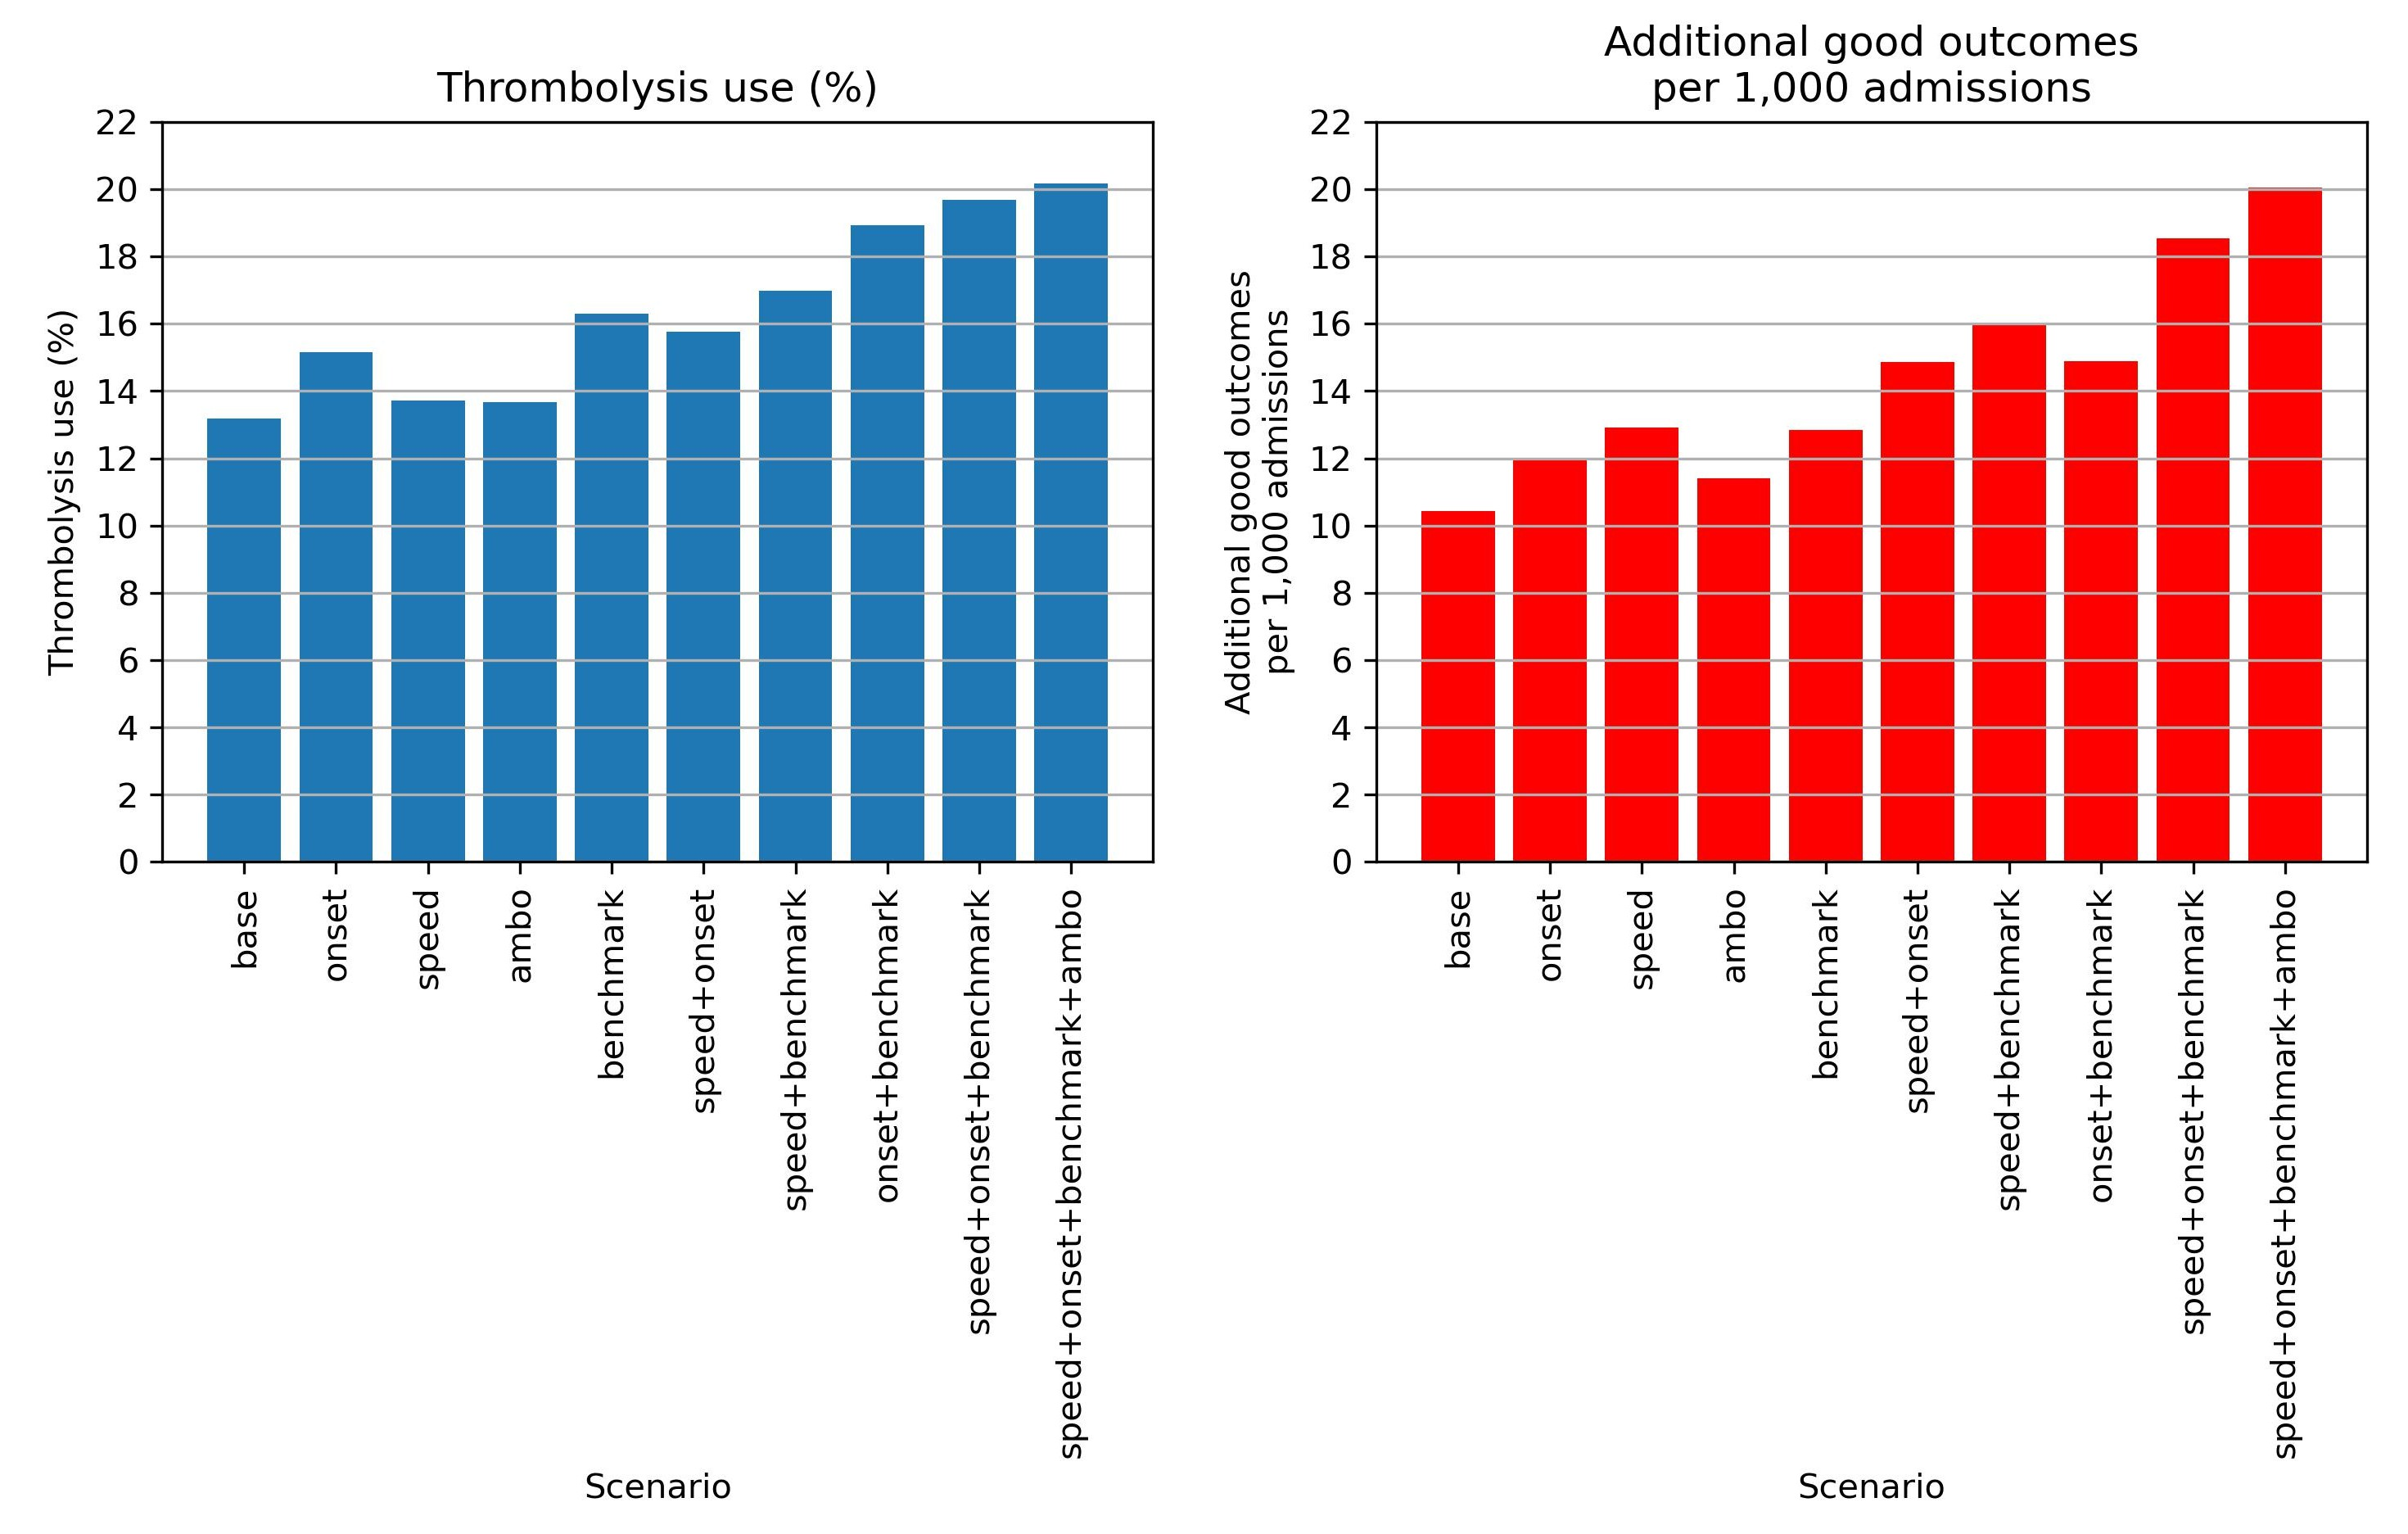
\includegraphics[width=1\linewidth]{images/p5_sim.jpg}
    \caption{Expected effect of alternative process improvement initiatives across the study population. The chart shows the effect on thrombolysis use (left) and on number of additional excellent outcomes (mRS 0-1) per 1,000 admissions due to use of thrombolysis (right). \textit{Base}: Uses the hospitals’ recorded pathway statistics. \textit{Onset}: Sets the proportion of patients with a known stroke onset time to the national upper quartile if currently less than the national upper quartile. \textit{Speed}: Sets 95\% of patients having a scan within 4 hours of arrival, and all patients have 15 minutes arrival-to-scan time and 15 minutes scan-to-needle time. \textit{Ambo}: Subtracts 15 minutes from the current ambulance call to arrival-at-hospital times. \textit{Benchmark}: The benchmark thrombolysis rate takes the likelihood to give thrombolysis for patients scanned within 4 hours of onset from the majority vote of the 25 benchmark hospitals.}
    \label{fig:scenarios_population}
\end{figure}

\FloatBarrier

\subsection{Lifetime economic model}

Table \ref{tab:health_econ} shows the modelled health economics of thrombolysis use, comparing actual use of thrombolysis with \textit{benchmark} thrombolysis use. The effect of thrombolysis was estimated by predicting the outcomes with and without thrombolysis for the two groups (those that actually received thrombolysis, and those predicted to receive thrombolysis using \textit{benchmark} decisions). Benchmark decisions maintain the benefit of using thrombolysis, but extend that benefit to more patients. This extended benefit was not at the cost of any predicted increase in the worst outcomes (mRS 5-6). The extended benefit led to more QALYs added across the population by treatment, and more predicted savings to NHS healthcare costs.

\begin{table}[!ht]
\small
\caption{Health economic analysis: Analysis for  populations based on predicted benefit (or dis-benefit) of thrombolysis. The effect of thrombolysis was estimated by predicting the outcomes with and without thrombolysis for the two groups (those that actually received thrombolysis, and those predicted to receive thrombolysis using \textit{benchmark} decisions). The analysis compares the populations currently treated, or the population that would be treated using \textit{benchmark} decisions (the majority vote of the predicted choice of the the 25 stroke teams most likely to use thrombolysis). Results are shown for (a) the treated populations, and (b) adjusted for 1,000 emergency stroke admissions }
\label{tab:main}

%\begin{subtable}{1\textwidth}
%\centering
%\caption{Analysis of the predicted effect of thrombolysis in two population subgroups: 1) those patients who actually received thrombolysis, or 2) those patients where the \textit{benchmark decision} would be to use thrombolysis. For each populations the outcomes with and without thrombolysis were predicted.}
%\begin{tabular}{p{2.0cm} p{1.5cm} p{1.2cm} p{1.3cm} p{1.5cm} p{1.3cm} p{1.4cm} p{1.3cm} p{1.3cm}}
%\toprule
%Modelled population & \raggedright Modelled treatment & Death & Survival (median years) & Care years (median) & QALYs & \raggedright Discounted cost per patient & Proportion mRS 0-2 & Proportion mRS 5-6\tabularnewline
%\midrule
%Actual use & Untreated & 17.1\% & 7.60 & 0.28 & 5.020 & £20,370 & 47.1\% & 23.9\%\tabularnewline
%& Treated & 14.2\% & 7.91 & 0.25 & 5.258 & £19,806 & 53.9\% & 19.3\%\tabularnewline
%& Difference & -2.9\% & 0.31 & -0.03 & 0.238 & -£565 & 6.8\% & -4.7\%\tabularnewline
%\midrule
%Benchmark & Untreated & 17.4\% & 7.63 & 0.28 & 5.036 & £20,388 & 46.5\% & 24.1\%\tabularnewline
%& Treated & 14.4\% & 7.93 & 0.25 & 5.269 & £19,784 & 53.4\% & 19.4\%\tabularnewline
%& Difference & -3.0\% & 0.30 & -0.03 & 0.234 & -£603 & 6.9\% & -4.8\%\tabularnewline
%\end{tabular}
%\end{subtable}

\vspace{3mm}

\begin{subtable}{1\textwidth}
\centering
\caption{Analysis for 1,000 emergency stroke admissions (all stroke types)}
\begin{tabular}{p{1.9cm} p{1.9cm} p{1.9cm} p{1.9cm} p{1.9cm} p{1.9cm} p{2.2cm}}
\toprule
Modelled population & Proportion treated & QALYs added & Healthcare costs saved & \raggedright Thrombolysis cost (£450 per patient) & \raggedright Cost per QALY added & \raggedright Net cost of thrombolysis\tabularnewline
\midrule
Actual & 11.0\% & 26.3 & £62,294 & £49,658 & £1,890 & -£12,637\tabularnewline
Benchmark & 13.6\% & 31.7 & £81,914 & £61,117 & £1,927 & -£20,797\tabularnewline
\bottomrule
\end{tabular}
\end{subtable}
\label{tab:health_econ}
\end{table}

\normalsize

\FloatBarrier

\subsection{Conclusions}

There is significant inter-hospital variation in use of thrombolysis that is caused by hospital processes and differences in decision-making. Improving processes and adopting the decision making of higher-thrombolysing units would be expected to increase thrombolysis use and has the potential to double the population benefit from thrombolysis. Higher-thrombolysing sites are delivering greater cost-effectiveness from thrombolysis through reductions in long-term disability in a greater number of patients.  Pathway analysis and machine learning should allow stroke teams to better understand, and improve, their own pathways.